\documentclass[sigconf]{acmart}

\usepackage{enumitem}
\usepackage{booktabs}
\usepackage{tabularx}
\usepackage{array}
\title[Academic Efficiency]{Academic Efficiency: Studying Better, Not Just More}
\subtitle{FAA - 2 Semester - 25/26 - Grupo x}

\author{Guilherme Soares}
\affiliation{%
  \institution{Faculty of Sciences of the University of Lisbon}
  \city{Lisbon}
  \country{Portugal}}
\email{fc62372@ciencias.ulisboa.pt}

\author{Vitória Correia}
\affiliation{%
  \institution{Faculty of Sciences of the University of Lisbon}
  \city{Lisbon}
  \country{Portugal}}
\email{fc62211@ciencias.ulisboa.pt}

\author{Duarte Soares}
\affiliation{%
  \institution{Faculty of Sciences of the University of Lisbon}
  \city{Lisbon}
  \country{Portugal}}
\email{fc62371@ciencias.ulisboa.pt}

\renewcommand{\shortauthors}{Soares G., Correia V. and Soares D.}
\acmConference{FAA - 2 Semester - 25/26 - Grupo x}{April 2026}{Lisbon, Portugal}
\begin{document}

\begin{teaserfigure}
  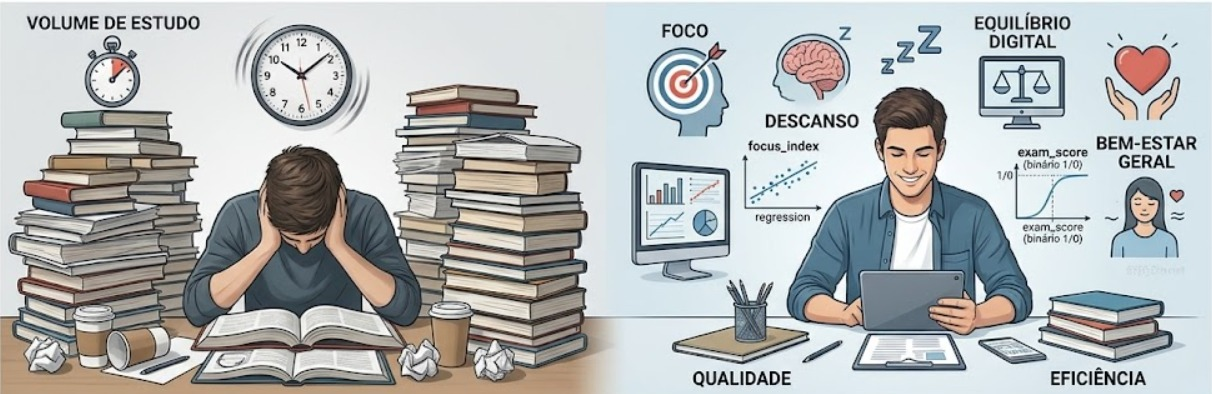
\includegraphics[width=\textwidth]{imagens/teaser.jpeg}
  \caption{Person struggling to study and studying happily (AI Generated), 2026.}
  \Description{A comparison between a stressed student and a focused, happy student studying.}
\end{teaserfigure}


\begin{abstract}
This project investigates academic efficiency in higher education, with the goal of understanding whether student success depends mainly on the amount of study time or on a broader combination of focus, rest quality, digital habits, and general well-being. Using a multidimensional student dataset, we define two complementary prediction tasks. The regression task aims to estimate students \texttt{focus\_index}, while the classification task predicts whether a student is likely to achieve a high \texttt{exam\_score}. 

To support these tasks, the data is preprocessed through a structured pipeline that handles missing values, categorical encoding, and feature scaling for mixed-type variables. Baseline interpretable models are first evaluated, followed by more complex approaches and hyperparameter optimization. In addition, unsupervised clustering is used to identify latent student profiles, and model interpretability techniques are applied to explain the most influential factors behind predictions. 

The project seeks to provide insight into how study-related and lifestyle-related behaviors contribute to academic efficiency, offering potential value for students, tutors, and academic support services.
\end{abstract}

\maketitle

\ccsdesc[500]{Computing methodologies~Machine learning}
\ccsdesc[300]{Computing methodologies~Supervised learning}
\ccsdesc[300]{Computing methodologies~Cluster analysis}
\ccsdesc[100]{Information systems~Data mining}

\keywords{academic efficiency, machine learning, supervised learning, regression, classification, clustering, student performance, focus prediction}

% =========================
% START OF REPORT
% =========================

\section{Introduction}

Academic performance has traditionally been associated with the amount of time students dedicate to studying. However, recent perspectives suggest that academic success is influenced by a broader set of factors, including focus, sleep quality, digital habits, and overall well-being \cite{walckiers2017students}. Understanding how these dimensions interact is therefore essential for promoting more efficient and sustainable learning strategies.

To explore the relationship between these variables and academic outcomes, this project will use of the dataset \texttt{student\_records\_missing.csv}, provided by the course instructors, which contains information about students' study habits, lifestyle, and performance indicators. We defined two complementary prediction tasks: a regression task aimed at estimating the \texttt{focus\_index}, and a classification task to predict whether a student is likely to achieve a high \texttt{exam\_score}. A complete machine learning pipeline is implemented, including data preprocessing, baseline model evaluation, advanced model optimization, and clustering analysis.

Additionally, model interpretability techniques are applied to better understand the factors that most influence predictions, and error analysis is conducted to identify limitations and potential improvements. The goal of this work is not only to build accurate predictive models, but also to derive meaningful insights that can support students, educators, and academic institutions in improving learning outcomes.


\section{Problem Definition}

\subsection{Problem Statement}

The main objective of this project is to investigate whether students' academic efficiency depends solely on the amount of time dedicated to studying, or if it results from a combination of factors such as focus, quality of rest, digital habits, and overall well-being. This problem is particularly relevant in modern educational contexts, where students are exposed to multiple sources of distraction and varying lifestyle patterns that may impact their academic performance.

\subsection{Target Variables}

To address the defined problem, two complementary predictive scenarios are considered.

\textbf{Regression Scenario:}  
The variable \texttt{focus\_index} is used as the target for regression, representing a continuous measure of a student's ability to maintain concentration during study activities.

\textbf{Classification Scenario:}  
The variable \texttt{exam\_score} is transformed into a binary target representing academic performance. Specifically, a threshold is defined to distinguish between high performance (1) and normal or low performance (0), allowing the problem to be framed as a classification task.

\subsection{Stakeholders}

Several stakeholders can benefit from the outcomes of this study.

\textbf{Students:}  
Students can gain insights into whether increasing study time alone leads to better performance, or if other factors such as focus and well-being play a more significant role.

\textbf{Mentors and Tutors:}  
Educators and tutors can use the findings to recommend more effective and personalized study strategies, focusing not only on study duration but also on behavioral and lifestyle factors.

\textbf{Academic Support Services:}  
Institutional support services can leverage these insights to design interventions aimed at improving academic success, emphasizing healthy habits, balanced digital usage, and overall student well-being rather than solely increasing study workload.



\section{Data Preprocessing Pipeline}
\subsection{Handling Missing Values}

The dataset used in this project contains missing values in both numerical and categorical features, which must be handled before training any machine learning model. Since most algorithms do not natively support missing data, leaving these values untreated could lead to errors or unreliable results, as discussed in the statistical learning literature \cite{hastie2009overview}.

Several strategies were considered, such as removing rows with missing values, discarding incomplete features, or relying on algorithms that can tolerate missing data. However, removing rows would reduce the amount of available data and could eliminate relevant patterns, while removing features might discard useful predictive information. For this reason, these alternatives were considered less appropriate for the present scenario.

Instead, a data imputation strategy was adopted in order to preserve the dataset while providing plausible estimates for missing values. The method was defined according to the type of feature:

\begin{itemize}
    \item \textbf{Numerical Features:} Missing values were imputed using the median. This choice is appropriate because the median is more robust to extreme values and skewed distributions, which are common in real-world datasets \cite{hastie2009overview}.
    
    \item \textbf{Categorical Features:} Missing values were imputed using the most frequent category (mode), ensuring that the replacement remains consistent with the observed distribution of each variable.
\end{itemize}

Although an initial cleaning step was carried out for exploratory and descriptive purposes, the final imputation process used for modelling was implemented inside a preprocessing pipeline with \textit{SimpleImputer}. This ensures that imputation parameters are learned only from the training data during cross-validation and then applied consistently to validation or test data, preventing data leakage. This practice follows standard recommendations for model evaluation procedures \cite{hastie2009model_assessment}.

\subsection{Categorical Encoding}

The dataset contains several categorical variables that must be converted into numerical format so they can be used by machine learning algorithms. Two main encoding approaches were considered: ordinal encoding and one-hot encoding.

Since the categorical features in this dataset do not have a natural order, ordinal encoding would introduce artificial relationships between categories. Therefore, one-hot encoding was selected as the most suitable strategy.

Using \textit{OneHotEncoder}, each category is transformed into a binary indicator variable, avoiding the introduction of any implicit ranking between categories. This approach is consistent with standard practices in statistical learning, where preserving the independence of categorical levels is important for model correctness \cite{hastie2009overview}.

In addition, the encoder was configured with \texttt{handle\_unknown="ignore"}, which improves robustness by allowing unseen categories in validation or test data to be processed without errors.

While one-hot encoding increases the dimensionality of the feature space, this trade-off is acceptable because it preserves the meaning of categorical information and supports the use of a broad range of machine learning models. This effect is related to the challenges of high-dimensional data discussed in the literature \cite{hastie2009high_dimensional}.

\subsection{Feature Scaling}

Feature scaling is important to ensure that numerical variables with different ranges do not disproportionately influence the learning process. This is especially relevant for algorithms that are sensitive to feature magnitude, such as support vector machines and regression-based methods, where distances and coefficient magnitudes directly affect the model \cite{hastie2009linear_regression}.

In this project, numerical features were scaled using \textit{RobustScaler}. Unlike standard normalization methods based on the mean and standard deviation, \textit{RobustScaler} centers the data using the median and scales it according to the interquartile range (IQR). This makes it more robust to outliers and better suited to datasets where numerical variables may contain extreme values or asymmetric distributions.

Scaling was applied only to numerical features, while categorical features were left unchanged after one-hot encoding. As with the other preprocessing steps, scaling was integrated into the pipeline so that all transformation parameters are estimated exclusively from the training data. This guarantees methodological correctness, prevents data leakage, and ensures consistency across all cross-validation folds \cite{hastie2009model_assessment}.

Overall, the preprocessing pipeline provides a structured and reproducible way of transforming the data, combining imputation, categorical encoding, and robust scaling into a single workflow suitable for fair and reliable model evaluation.

\subsection{Comparison of the Dataset Before and After Preprocessing}

To evaluate the impact of the preprocessing pipeline, a detailed comparison was conducted between the dataset before and after transformation. This analysis focuses on dataset dimensionality, missing-value treatment, and the structure of the resulting feature space.

Before preprocessing, the dataset contained 5000 instances and 16 features. A total of 2150 missing values were identified across both numerical and categorical variables. After applying the preprocessing pipeline, all missing values were handled through imputation, and the dataset was transformed into a fully numerical representation with 22 features.

The number of instances remained unchanged, indicating that no observations were removed during preprocessing. The increase in dimensionality is explained by the application of one-hot encoding to categorical variables, which expands the feature space in exchange for improved representational capacity \cite{hastie2009high_dimensional}.

\begin{table}[t]
\centering
\caption{Dataset structure before and after preprocessing}
\begin{tabular}{lcc}
\toprule
\textbf{Stage} & \textbf{Rows} & \textbf{Columns} \\
\midrule
Before preprocessing & 5000 & 16 \\
After preprocessing  & 5000 & 22 \\
\bottomrule
\end{tabular}
\end{table}

Missing values were present in several variables prior to preprocessing, particularly in \textit{mental\_health\_score}, \textit{caffeine\_intake\_mg}, and \textit{screen\_time\_hours}. After applying median imputation for numerical variables and mode imputation for categorical variables, all missing values were successfully removed.

\begin{table}[t]
\centering
\caption{Missing values before and after preprocessing}
\begin{tabular}{lcc}
\toprule
\textbf{Feature} & \textbf{Before} & \textbf{After} \\
\midrule
gender & 150 & 0 \\
academic\_level & 100 & 0 \\
social\_media\_hours & 250 & 0 \\
screen\_time\_hours & 400 & 0 \\
caffeine\_intake\_mg & 500 & 0 \\
mental\_health\_score & 750 & 0 \\
\midrule
\textbf{Total} & \textbf{2150} & \textbf{0} \\
\bottomrule
\end{tabular}
\end{table}

The categorical variables contain a small number of distinct categories, making them suitable for one-hot encoding.

\begin{table}[t]
\centering
\caption{Summary of categorical features before preprocessing}
\begin{tabular}{lcccc}
\toprule
\textbf{Variable} & \textbf{Count} & \textbf{Missing} & \textbf{Unique} & \textbf{Mode} \\
\midrule
gender & 4850 & 150 & 3 & Male \\
academic\_level & 4900 & 100 & 3 & Postgraduate \\
internet\_quality & 5000 & 0 & 3 & Good \\
\bottomrule
\end{tabular}
\end{table}

After preprocessing, categorical variables were transformed using one-hot encoding, resulting in binary indicator features.

\begin{table*}[t]
\centering
\caption{Categorical features after preprocessing (one-hot encoded)}
\begin{tabular}{lcccc}
\toprule
\textbf{Variable} & \textbf{Count} & \textbf{Missing} & \textbf{Unique} & \textbf{Mode} \\
\midrule
cat\_\_gender\_Female & 5000 & 0 & 2 & 0 \\
cat\_\_gender\_Male & 5000 & 0 & 2 & 0 \\
cat\_\_gender\_Other & 5000 & 0 & 2 & 0 \\
cat\_\_academic\_level\_High School & 5000 & 0 & 2 & 0 \\
cat\_\_academic\_level\_Postgraduate & 5000 & 0 & 2 & 0 \\
cat\_\_academic\_level\_Undergraduate & 5000 & 0 & 2 & 0 \\
cat\_\_internet\_quality\_Average & 5000 & 0 & 2 & 0 \\
cat\_\_internet\_quality\_Good & 5000 & 0 & 2 & 0 \\
cat\_\_internet\_quality\_Poor & 5000 & 0 & 2 & 0 \\
\bottomrule
\end{tabular}
\end{table*}

Each encoded feature contains only values in $\{0,1\}$, indicating the absence or presence of a given category. The mode of each variable is 0, reflecting that for each observation, only one category per original feature is active.

\begin{table*}[t]
\centering
\caption{Summary of numerical features before preprocessing}
\begin{tabular}{lccccccc}
\toprule
\textbf{Variable} & \textbf{Count} & \textbf{Missing} & \textbf{Mean} & \textbf{Std} & \textbf{Min} & \textbf{Median} & \textbf{Max} \\
\midrule
age & 5000 & 0 & 20.520 & 2.870 & 16.0 & 20.000 & 25.00 \\
study\_hours & 5000 & 0 & 4.540 & 1.822 & 0.0 & 4.530 & 11.84 \\
self\_study\_hours & 5000 & 0 & 2.479 & 1.178 & 0.0 & 2.480 & 7.41 \\
online\_classes\_hours & 5000 & 0 & 2.012 & 0.984 & 0.0 & 2.010 & 6.00 \\
social\_media\_hours & 4750 & 250 & 2.995 & 1.467 & 0.0 & 2.975 & 8.28 \\
gaming\_hours & 5000 & 0 & 1.565 & 1.111 & 0.0 & 1.490 & 5.64 \\
sleep\_hours & 5000 & 0 & 7.016 & 1.164 & 4.0 & 7.010 & 10.00 \\
screen\_time\_hours & 4600 & 400 & 6.986 & 2.476 & 1.0 & 6.955 & 15.30 \\
exercise\_minutes & 5000 & 0 & 74.536 & 42.932 & 0.0 & 75.000 & 149.00 \\
caffeine\_intake\_mg & 4500 & 500 & 251.127 & 143.810 & 0.0 & 251.000 & 499.00 \\
part\_time\_job & 5000 & 0 & 0.498 & 0.500 & 0.0 & 0.000 & 1.00 \\
upcoming\_deadline & 5000 & 0 & 0.501 & 0.500 & 0.0 & 1.000 & 1.00 \\
mental\_health\_score & 4250 & 750 & 5.505 & 2.866 & 1.0 & 6.000 & 10.00 \\
\bottomrule
\end{tabular}
\end{table*}

After preprocessing, numerical features were scaled using RobustScaler.

\begin{table*}[t]
\centering
\caption{Numerical features after preprocessing}
\begin{tabular}{lccccccc}
\toprule
\textbf{Variable} & \textbf{Count} & \textbf{Missing} & \textbf{Mean} & \textbf{Std} & \textbf{Min} & \textbf{Median} & \textbf{Max} \\
\midrule
num\_\_age & 5000 & 0 & 0.104 & 0.574 & -0.800 & 0.0 & 1.000 \\
num\_\_study\_hours & 5000 & 0 & 0.004 & 0.726 & -1.805 & 0.0 & 2.912 \\
num\_\_self\_study\_hours & 5000 & 0 & -0.001 & 0.723 & -1.521 & 0.0 & 3.025 \\
num\_\_online\_classes\_hours & 5000 & 0 & 0.001 & 0.718 & -1.467 & 0.0 & 2.912 \\
num\_\_social\_media\_hours & 5000 & 0 & 0.010 & 0.749 & -1.558 & 0.0 & 2.777 \\
num\_\_gaming\_hours & 5000 & 0 & 0.045 & 0.665 & -0.892 & 0.0 & 2.485 \\
num\_\_sleep\_hours & 5000 & 0 & 0.004 & 0.740 & -1.914 & 0.0 & 1.901 \\
num\_\_screen\_time\_hours & 5000 & 0 & 0.009 & 0.759 & -1.903 & 0.0 & 2.666 \\
num\_\_exercise\_minutes & 5000 & 0 & -0.006 & 0.572 & -1.000 & 0.0 & 0.987 \\
num\_\_caffeine\_intake\_mg & 5000 & 0 & 0.001 & 0.623 & -1.146 & 0.0 & 1.132 \\
num\_\_part\_time\_job & 5000 & 0 & 0.498 & 0.500 & 0.000 & 0.0 & 1.000 \\
num\_\_upcoming\_deadline & 5000 & 0 & -0.499 & 0.500 & -1.000 & 0.0 & 0.000 \\
num\_\_mental\_health\_score & 5000 & 0 & -0.084 & 0.530 & -1.000 & 0.0 & 0.800 \\
\bottomrule
\end{tabular}
\end{table*}

\begin{table}[h]
\centering
\caption{Feature composition after preprocessing}
\begin{tabular}{lc}
\toprule
\textbf{Feature group} & \textbf{Number of features} \\
\midrule
Scaled numerical features & 13 \\
One-hot encoded categorical features & 9 \\
\midrule
\textbf{Total transformed features} & \textbf{22} \\
\bottomrule
\end{tabular}
\end{table}

Overall, the preprocessing pipeline produced a complete, numerically consistent, and machine-learning-ready dataset. The elimination of missing values, combined with appropriate encoding and scaling techniques, ensures that subsequent model evaluation is conducted on reliable and well-structured data.

\section{Baseline Models}

Nesta fase, foram estabelecidos modelos de referência para definir o desempenho, focando em algoritmos interpretáveis antes da transição para abordagens mais complexas.

\subsection{Regression Task}
Para a estimativa do \texttt{focus\_index}, utilizou-se a Regressão Linear como modelo base. A escolha justifica-se pela necessidade de compreender a relação direta entre hábitos de estudo e capacidade de foco. Como complemento, aplicou-se uma Árvore de Decisão (\texttt{max\_depth=5}) para verificar se existem relações não lineares simples que o modelo linear possa omitir. A comparação quantitativa validou a Regressão Linear como o modelo de referência mais estável.

\subsection{Classification Task}
Para a tarefa de classificação (\texttt{high\_exam\_score}), implementou-se a Regressão Logística e uma Árvore de Decisão. O modelo de Regressão Logística foi configurado com \texttt{class\_weight="balanced"} para compensar o desequilíbrio das classes ($\approx 25\%$ de positivos). Este modelo revelou-se a \textit{baseline} de eleição, demonstrando uma capacidade discriminativa superior face à árvore de decisão, que apresentou sinais de \textit{overfitting} nos dados de treino.

\subsection{Evaluation Metrics}
As métricas de sucesso foram definidas para permitir uma avaliação rigorosa:
\begin{itemize}
    \item \textbf{Regressão:} O \textit{Root Mean Squared Error} (RMSE) foi a métrica primária, dada a penalização mais severa em erros elevados. O \textit{Mean Absolute Error} (MAE) serviu como métrica secundária para uma interpretação direta do erro médio.
    \item \textbf{Classificação:} O \textit{F1-score} foi selecionado como métrica primária para equilibrar \textit{precision} e \textit{recall} num cenário de classes desbalanceadas. A \textit{ROC-AUC} foi utilizada como métrica secundária para avaliar a capacidade discriminativa do modelo independentemente do \textit{threshold} de decisão.
\end{itemize}

\section{Feature Engineering and Selection}

\section{Advanced Models and Hyperparameter Tuning}

\subsection{Model Selection}

\subsection{Hyperparameter Optimization}


\section{Unsupervised Learning (Clustering)}
Nesta etapa, procedeu-se à identificação de subgrupos latentes na população estudantil. O objetivo foi agrupar estudantes com perfis comportamentais e de bem-estar semelhantes, sem o recurso a variáveis-alvo, permitindo uma descoberta de padrões puramente baseada nos atributos observados.

\subsection{Cluster Selection}
Para a execução do algoritmo K-Means, os dados foram pré-processados e normalizados através do \texttt{StandardScaler}, garantindo que a escala das variáveis não influenciasse indevidamente o cálculo das distâncias euclidianas. 
A determinação do número ideal de clusters ($k$) foi realizada através da combinada de duas heurísticas matemáticas:
\begin{figure}
    \centering
    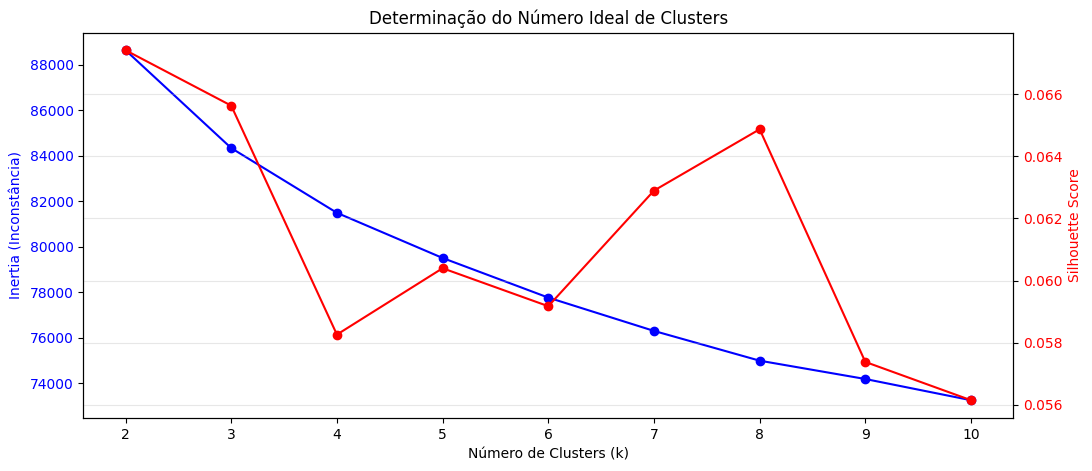
\includegraphics[width=1\linewidth]{imagens/k_clusters.png}
    \caption{Analysis of cluster centers based on student behaviors. Source: Authors' own work (2026).}
    \label{fig:k_clusters}
\end{figure}
\begin{itemize}
    \item \textbf{Método Elbow (Inércia):} Observou-se a variação da inércia em função de $k$ para identificar o ponto de inflexão na redução da variância intra-cluster.
    \item \textbf{Silhouette Score:} Calculou-se o coeficiente de silhueta para medir a coesão e separação entre clusters.
\end{itemize}
Após a análise gráfica, da figura ~\ref{fig:k_clusters}, fixou-se $k=8$ como o número ótimo, apresentando o melhor compromisso entre a redução da inércia e a manutenção de uma separação clara entre os perfis estudantis.
\subsection{Cluster Interpretation}
A análise dos centroides permitiu a construção de "personas" estudantis, interpretando as médias dos atributos por cluster em relação à média global da população. Esta interpretação revelou padrões comportamentais distintos:
\sloppy
\begin{itemize}
    \item \textbf{O Procrastinador Descansado (Cluster 0, alto: caffeine\_intake\_mg, sleep\_hours; baixo: study\_hours, exercise\_minutes):} Estudante que dorme muito e consome cafeína, mas apresenta pouco tempo de estudo e exercício.
    \item \textbf{O Atleta Zen (Cluster 1, alto: exercise\_minutes, mental\_health\_score; baixo: social\_media\_hours, caffeine\_intake\_mg):} Muito ativo fisicamente, com excelente saúde mental e afastado das redes sociais.
    \item \textbf{O Ativo Digitalmente Exausto (Cluster 2, alto: exercise\_minutes, screen\_time\_hours; baixo: mental\_health\_score, caffeine\_intake\_mg):} Fisicamente ativo, mas com a saúde mental desgastada pelo uso excessivo de ecrãs.
    \item \textbf{O Sedentário Digital (Cluster 3, alto: screen\_time\_hours, social\_media\_hours; baixo: exercise\_minutes, caffeine\_intake\_mg):} Foco total em redes sociais e ecrãs, sem qualquer prática de exercício físico.
    \item \textbf{O Veterano Conectado (Cluster 4, alto: age, social\_media\_hours; baixo: exercise\_minutes, caffeine\_intake\_mg):} Estudante de idade mais avançada, muito ativo no mundo digital, mas com baixa atividade física.
    \item \textbf{O Rato de Biblioteca Cafeinado (Cluster 5, alto: caffeine\_intake\_mg, self\_study\_hours; baixo: upcoming\_deadline, screen\_time\_hours):} Dedicado ao estudo autónomo e ao consumo de café, com reduzido tempo de exposição a ecrãs.
    \item \textbf{O Veterano Aplicado (Cluster 6, alto: age, study\_hours; baixo: exercise\_minutes, caffeine\_intake\_mg):} Estudante mais velho com carga de estudo elevada, sedentário e sem dependência de cafeína.
    \item \textbf{O Focado Produtivo (Cluster 7, alto: caffeine\_intake\_mg, mental\_health\_score; baixo: sleep\_hours, screen\_time\_hours):} Consumo elevado de cafeína, poucas horas de sono e ecrã, mas mantendo uma saúde mental resiliente.
\end{itemize}
\fussy
Estes perfis demonstram que a população estudantil não é homogénea, existindo ecossistemas comportamentais únicos que influenciam a vivência académica, independentemente dos resultados diretos nas avaliações.

\section{Model Interpretability}

\section{Error Analysis}

\section{Results and Discussion}

\section{Conclusion}

At this stage, the first part of the project has been completed, including problem definition, data understanding, and the construction of a preprocessing pipeline suitable for both regression and classification tasks. The results obtained so far show that the dataset was successfully cleaned and transformed into a consistent format for machine learning, ensuring methodological correctness and preventing data leakage. Although the predictive modelling, optimization, clustering, and interpretability stages are still under development, this initial phase already provides a solid foundation for the next steps of the project. The remaining work will focus on evaluating models and extracting meaningful insights about the factors that contribute most to academic efficiency.

% =========================
% BIBLIOGRAPHY
% =========================

\bibliographystyle{ACM-Reference-Format}
\bibliography{references}

\end{document}